%!TEX root =  IdmxSpecification.tex

\section{Architecture Overview}
\label{sec:arch}

The Idmx library contains a crypto engine for each role that an entity may assume.
Those engines share a common structure and code base and they 
can be divided into (1) a layer that assembles data and prepares it and
(2) an engine that coordinates the proof generation, and (3) a collection of abstract building blocks and 
their concrete implementations.
Figure~\ref{fig:overview} shows the those layers and the components that they consist of.
%
The first layer consists of all (signleton) orchestration objects for key generation, issuance, and 
proof generation,
the building block factory, and in general all singleton objects which do not involve zero knowledge proofs.
%
During presentation (or the presentation phase of an issuance), this first layer
receives as input a presentation token description (see~\cite{abc4trust:h22} for a detailed specification)
and a list of credentials;
it outputs a mechanism specification, and a list of objects (ZkModules) that will be needed for the proof
and which serves as input to the second layer.
This layer is responsible for assembling all the parameters (keys, configurations, etc.) required
by the various building blocks, and is responsible for
setting up the specified implementation for each given cryptographic primitive (e.g., CL-signatures as 
signature algorithm).
%
This layer delegates the generation of keys or parameters to the appropriate building block.


\begin{figure}[htbp]
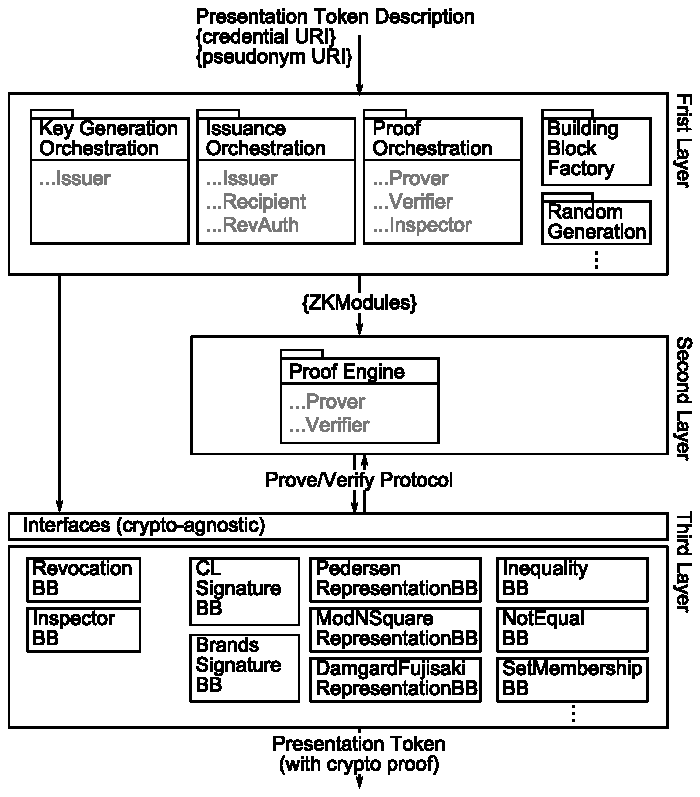
\includegraphics[width=\textwidth]{img/idmx_overview.pdf}
\caption{Visualization of the layers of the Identity Mixer architecture.
Note that singleton objects are denoted with a little box on top.}
\label{fig:overview}
\end{figure}

The second layer consists of the so called \emph{proof engine}. It receives as input a list of
ZkModules from the first layer
and generates/verifies a Fiat-Shamir zero-knowledge proof (``signature of knowledge'').
For the generation of keys, this layer is skipped and the orchestration object directly invokes the 
appropriate building block (i.e., a signature building block).


In the third layer, the abstract building blocks
only expose implementation-agnostic interfaces.
The implementations thereof know how to perform a specific cryptographic primitive, but do
not necessarily know how to interact with other primitives.
%
In general, building
blocks consist of one of more key/parameter generators, and of one
or more proof interfaces (\emph{ZkModules} factories).
%
Roughly speaking, ZkModules either (1) encapsulate the implementation of a given 
cryptographic primitive and expose a
crypto-primitive-agnostic interface to the proof engine;
or (2) have a structural role in the proof generation by indicating properties of attributes, 
relationships among attributes,
or adding messages to be signed.



\subsection{Parameter Generation}
\label{sec:arch:setup}

Let us describe the setup of parameters such as the system parameters, 
verifier parameters, or a key pair.
%
This is a two step process consisting of (1) creating a configuration template that has to 
be completed and submitted to (2) the generation of the set of parameters.
%
First, the user of the Idmx library starts by requesting a new (default) configuration template
from the crypto engine.
%
The request is forwarded to the key generation orchestration singleton object.
%
The orchestration element gathers all relevant data from the key manager 
before it
queries all relevant building blocks for the implementation specific configuration 
parameters that need to be added to the template.
%
The default configuration template is returned to the caller.


While a template is configured with default values that serve as
suggestion for a general purpose use, the actual settings must be set manually and 
in accordance with the planned use.
Note, only the general entries as well as the entries corresponding to the chosen 
implementation must be filled out in the template.
The entries
corresponding to non-chosen implementations will be ignored. 
%
We call the completed configuration template a configuration.



The second step starts with the user passing the configuration to the crypto engine, 
which forwards it to the 
orchestration object.
The latter, as in the creation of the configuration template, assembles the required  
parameters and forwards the data to the relevant 
building block corresponding to the chosen implementation.
Finally, the building block generates the requested parameters upon which they are 
returned to the requester.


\begin{figure}[htbp]
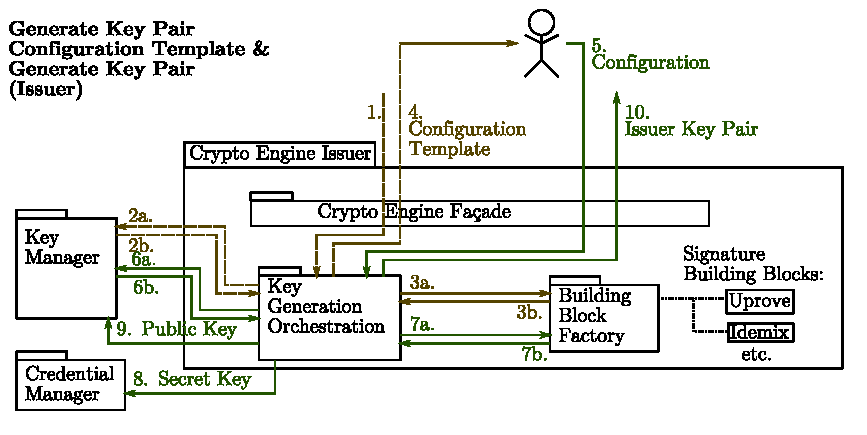
\includegraphics[width=\textwidth]{img/23.pdf}
\caption{Example of generating an issuer key pair including the creation of the 
corresponding key pair configuration template. Note that most objects in this figure 
with the exception of the concrete building blocks are singletons. This is indicated 
by the shape of their boxes.}
\label{fig:issuerkeypair}
\end{figure}

In Figure~\ref{fig:issuerkeypair} we depict the setup of an issuer key pair as an example 
of the parameter generation process. 
As mentioned before, the generation of system parameters, verifier parameters, or the
key pair of other entities is identical with the exception of a different set of
building blocks being queried. 

The user initiates with the request of a key pair configuration template (1) from the crypto 
engine.
%
Upon being forwarded to the orchestration object, the latter requests the system parameters 
from the key manager (2) as well as all signature building blocks from the building block
factory (3).
%
Further, it adds a few default entries to the configuration template, and asks each 
signature building block
in turn to add its own implementation-specific entries to the configuration template. 
The configuration
template is then returned to the user (4).


After finishing the configuration by overriding the appropriate default settings of the 
template configuration the user calls the crypto engine again with the request of generating
the parameters (5).
%
The key orchestration queries the key manager for the system parameters again (6), and the 
building
block factory for the chosen building block (7). 
It then asks the chosen building block to generate
an issuer key pair based on the configuration. 
Finally, the whole key pair is returned to the requester (10).
%
Note that the ABC4Trust adapter stores the secret key of that pair to the credential manager (8),
and the public key to the key manager (9). 


\subsection{Presentation}
\label{sec:arch:presentation}

Let us now illustrate the generation of a presentation token as depicted in 
Figure~\ref{fig:presentation}.
%
% TODO add verifier parameters
When a user wants to create a presentation token she needs to pass the presentation token
description,  a list of credential URIs, and a list of pseudonym URIs 
to the crypto engine.
%
These elements get forwarded to the proof orchestration object (1).
The proof orchestration first fetches the credentials and pseudonyms based on their URI from the
credential manager (2). 
Second, it loads the system parameters, issuer public keys, credential templates, inspector
public keys, and revocation authority public keys from the key manager (3).
Third, it queries the building block factory for the building blocks required for the presentation
token at hand (4).
For building blocks that have several implementations, the proof orchestration 
may choose a specific implementation, or it may ask the building block factory for
an implementation that is supported by the verifier.

\begin{figure}[htbp]
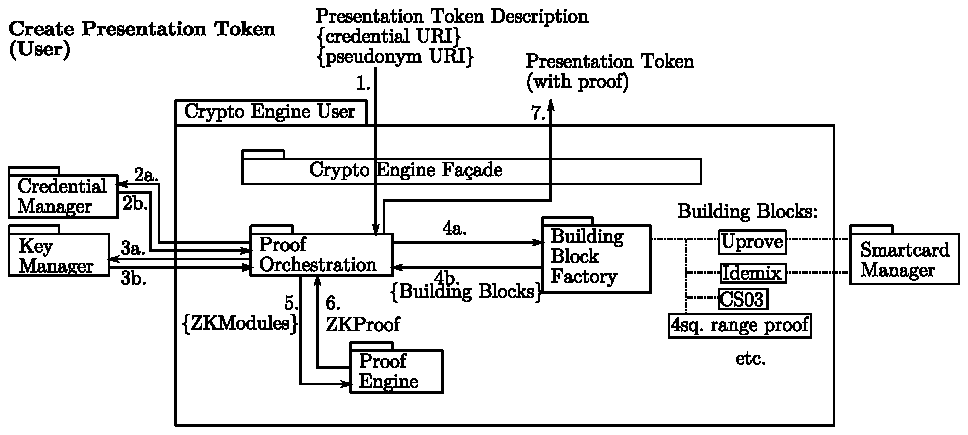
\includegraphics[width=\textwidth]{img/01.pdf}
\caption{Creation of a presentation token.}
\label{fig:presentation}
\end{figure}

These building blocks are used to generate a list of ZkModules that serve as input
to the proof engine (5).
%
The proof orchestration object will configure each ZkModule with the appropriate 
parameters such as the  keys, credentials, or pseudonyms.
The latter builds  a way of encapsulating the state needed to perform part of the overall 
zero-knowledge proof.
Note that ZkModules responsible for
proving ownership of a credential or a pseudonym may delegate part of the proof process 
to the smartcard manager.
The latter interacts with the smartcard to generate the proof elements contributed by a 
user-owned smartcard.
%
The proof engine generates a zero-knowledge proof (6) supporting the validity of the 
presentation token based on this list of ZkModules.
%
Using the proof, the orchestration object updates the presentation token description 
and then combines the former with the zero-knowledge
proof to form the final presentation token (7).




\subsection{Verification}
\label{sec:arch:verification}


Matching the presentation token to a presentation policy (as per ABC4Trust specifications) needs
to be performed before the former can be sent to the crypto engine for 
cryptographic verification (1).
%
The crypto engine forwards the
presentation token to the proof verification orchestration object, which fetches
the relevant system parameters, issuer public keys, credential
templates, inspector public keys, and revocation authority public keys from the key manager (2).


\begin{figure}[htbp]
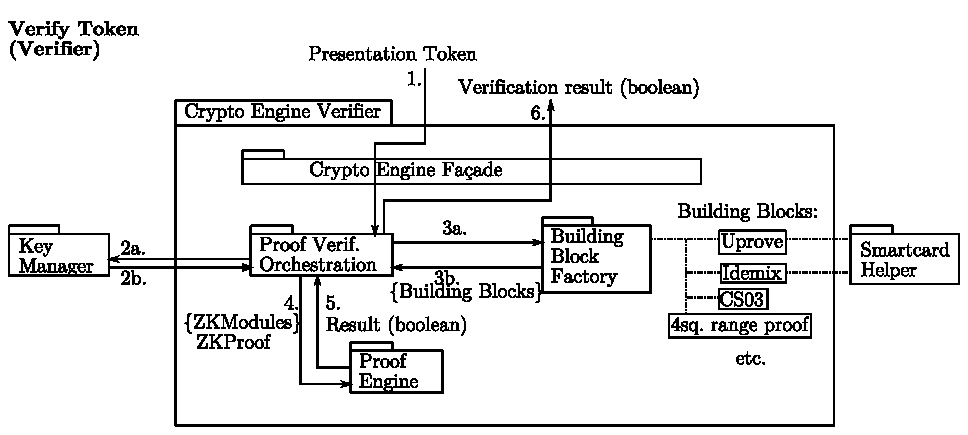
\includegraphics[width=\textwidth]{img/11.pdf}
\caption{Verification of a presentation token.}
\label{fig:verification}
\end{figure}


The verification orchestration needs to fetch the 
same set of building blocks from the building block factory (3) as the prover did.
To that end, the orchestration object uses the mechanism specification that describes the 
concrete implementations that have been chosen for each building block.
Thereafter, it can 
generate a list of ZkModules using these building blocks, where the ZkModules correspond 
to the list generated by the prover (4).
ZkModules together with the zero-knowledge proof are sent to the proof engine for 
verification.
Note that the verifier makes use of the smartcard helper, which is not connected to a smart card
but provides the functionality required to verify the part of the proof generated by a smart card.
The result of the verification (5) is then forwarded to the calling entity (6).





\subsection{Issuance}
\label{sec:arch:issuance}

We describe the issuance process in the case where no jointly-random attributes are present
and where the signing of the credential needs one round (as is the case for CL signatures).
%
Note, the issuance protocol continues for as many rounds as the used signature building block
specified and it reaches its end when the issuer specifies that it has sent the protocol 
ending message. 
%
Figure~\ref{fig:issuance1} and \ref{fig:issuance3} describe the process on the issuer's side
and Figure~\ref{fig:issuance2} and \ref{fig:issuance4} focus on the recipient of the 
credential.



\subsubsection{Issuer: Create Issuance Policy} 

On the level of the Idmx library (Fig.~\ref{fig:issuance1}), the issuance process starts with  the issuer invoking the crypto engine 
with an issuance policy and a list of issuer-set attributes (1), which 
are passed to the issuance orchestration object.
The latter saves the issuance policy and list of attributes in the state storage (2),
wraps the issuance policy in an issuance message, and returns that message to the upper layer (3).

\begin{figure}[htbp]
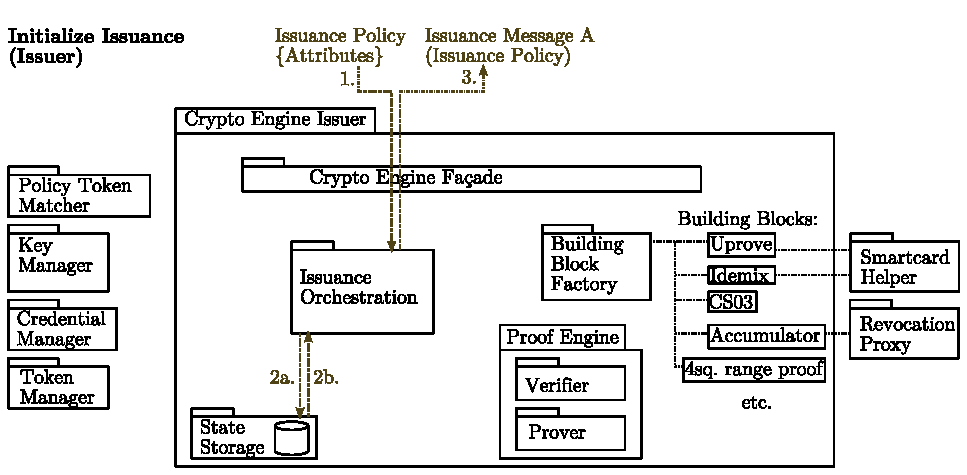
\includegraphics[width=\textwidth]{img/12.pdf}
\caption{Initiation of the issuance process on the issuer's side.}
\label{fig:issuance1}
\end{figure}




\subsubsection{Recipient: Generate Issuance Token} 

Figure~\ref{fig:issuance2} shows the recipient's side where the issuance token description, 
a list of credential URIs, a list of Pseudonym URIs, 
and the original issuance message need to be provided to the crypto engine (4).
%
These elements are forwarded to the issuance orchestration, which checks with the state storage that
the issuance context has never been seen before (5). 
Steps (6) to (10) are similar to a presentation proof (see Section~\ref{sec:arch:presentation}), with the exception of the 
issuance orchestration object additionally generating a ZkModule for carry-over from the signature building block.

\begin{figure}[htbp]
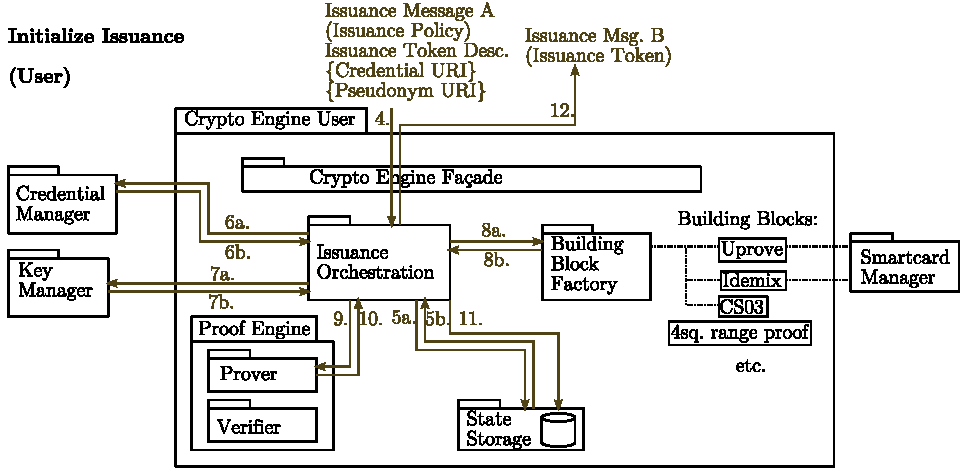
\includegraphics[width=\textwidth]{img/03.pdf}
\caption{Recipient computes an issuance token proving properties used for the credential to be issued.}
\label{fig:issuance2}
\end{figure}

After recovering the carry-over state from the proof received from the proof engine (10), orchestration 
generates an issuance token and the corresponding issuance token description, wraps the issuance token in
an issuance message, saves its current state in the state storage (11), and returns the issuance message 
to upper layer (12).




\subsubsection{Issuer: Create Signature}

The user's issuance message (containing the issuance token) is processed directly by the issuer's crypto engine.
It is passed to the issuance orchestration object (13), which recovers the state associated with the 
issuance context from the state storage (14). 
% HERE
%The issuance manager now asks the policy token Matcher from the ABC layer to check the issuance token against the
%original issuance policy (15). 
In steps (15) to (18) the issuance orchestration proceeds as the proof verification orchestration (see Section~\ref{sec:arch:verification})
to check the proof on the user's issuance token.

\begin{figure}[htbp]
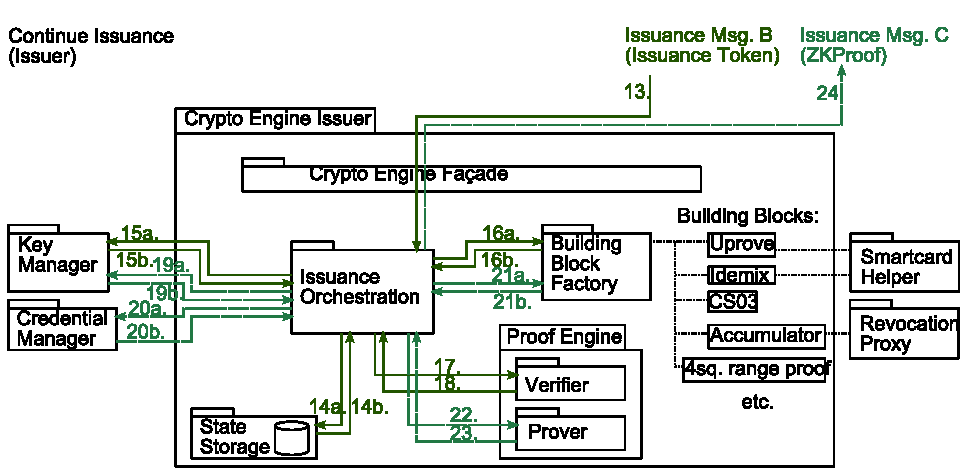
\includegraphics[width=\textwidth]{img/14a.pdf}
\caption{Issuer creates signature.}
\label{fig:issuance3}
\end{figure}


The issuance orchestration now recovers the revocation authority's public key from the key manager (19), the issuer's secret key
from the credential manager (20), and a building block for revocation of the correct implementation from the building block factory (21).
It then extracts the carry-over state from the ZkModule for carry-over and  generates a ZkModule for issuance from the
signature building block, which it initializes with the carry-over state, the issuer-set attributes, and the secret key.
If the credential that will be issued is revocable, it also generates a ZkModule for issuance from the building block for revocation.
During this step, the revocation authority will be contacted through the revocation proxy to retrieve a new revocation handle 
and the associated non-revocation evidence.
It then passes these two ZkModules to the proof engine (22).


During the proof generation, the ZkModule for signature issuance will actually perform the signature on the credential.
The issuance orchestration recovers the zero-knowledge proof from the proof engine (23). 
This zero-knowledge proof includes
the issuer's signature, the issuer-set attributes, the revocation handle, and the non-revocation evidence.
The orchestration object then queries the ZkModule for signature issuance for the list of attributes it knows about (including the revocation handle),
generates an issuance log entry.
% , and asks the ABC-layer token manager to save that log entry (26).
Finally, the zero-knowledge proof is wrapped into an issuance message, and returned to the requester (24).




\subsubsection{Recipient: Complete Signature}

The issuer's issuance message (containing the zero-knowledge proof) is processed directly by the user's crypto engine 
by passing it to the issuance orchestration object (28). 
The latter recovers the state associated with the issuance context from the state storage (29). 
It retrieves the necessary parameters, specifications and keys from the key manager (30).
Further, the orchestration loads a building block for signatures and a building block for revocation of the appropriate implementation from
the building block factory (31).

\begin{figure}[htbp]
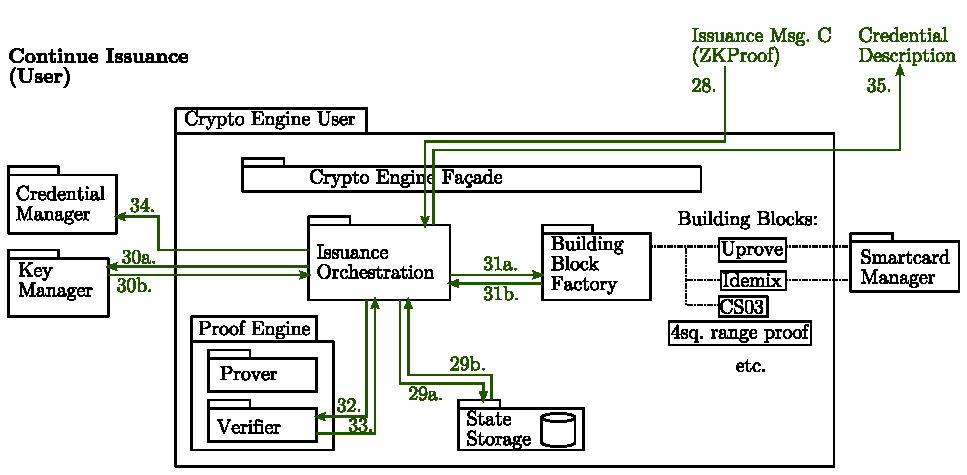
\includegraphics[width=\textwidth]{img/04.pdf}
\caption{Recipient finishes signature and stores credential.}
\label{fig:issuance4}
\end{figure}

The issuance orchestration gets a ZkModule for signature issuance from the first building block, initializing it with its
carry-over state and the issuer's public key. It also gets a ZkModule for revocation issuance from the second building block.
It then sends these two ZkModules and the zero-knowledge proof to the proof engine for verification (32).
After the issuance orchestration gets back the results of the proof verification (33), it extracts the issuance state from the
ZkModule for signature issuance. 
The issuance state can be combined with the carry-over state to recover the signed credential
and non-revocation evidence. 
The signed credential is saved in the credential manager (34). The issuance orchestration returns
the credential description to the upper layer (35).






